\begin{frame}[t]{Unidade básica de armazenamento}
    \transboxout[duration=0.5]
    \framesubtitle{Shell - Bits mecânicos}
    \begin{columns}
        \column{.1\textwidth}
        \column{.4\textwidth}
            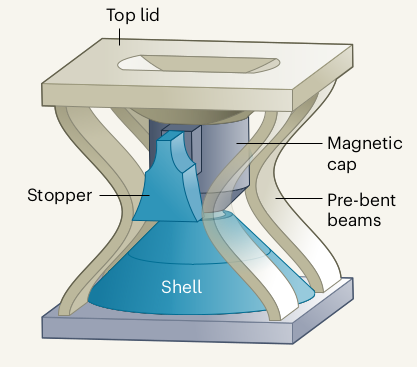
\includegraphics[width=.87\textwidth]{shell.png}
        \column{.6\textwidth}
            \begin{itemize}
                \item Conchas\footnote{Tradução livre de \textit{shell}.} que possuem uma instabilidade no seu encaixe.
                \item O encaixe pode ser controlado remotamente por um campo magnético externo.
            
            \end{itemize}
    \end{columns}
    
    \note[item]{Somente duas posições possuem estabilidade em sua configuração.}
\end{frame}

\begin{frame}[t]{Unidade básica de armazenamento}
    \transboxout[duration=0.5]
    \framesubtitle{Funcionamento}
    %\transboxin[duration=1,direction=30]
    
    \begin{figure}
        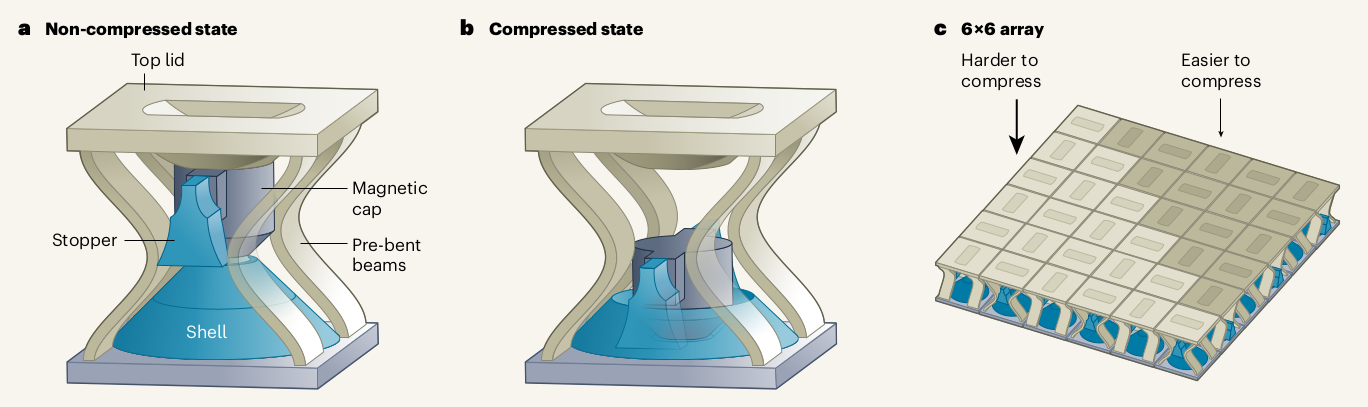
\includegraphics[width=1\textwidth]{shell-work.png}
        %\caption{.}
    \end{figure}
    \small
    A tampa magnética conduz o processo de encaixe, este que por sua vez determina a compressibilidade do ponto. 
%*----------- notes
    \note[item]{Notes can help you to remember important information. Turn on the notes option.}
\end{frame}

\begin{frame}[t]{Unidade básica de armazenamento}
    \transboxout[duration=0.5]
    \framesubtitle{Processo de gravação}
    \begin{columns}
        % \column{.1\textwidth}
        \column{.4\textwidth}
            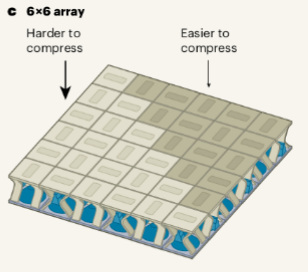
\includegraphics[width=.87\textwidth]{shell-array.png}
        \column{.5\textwidth}
        Utilizando um dispositivo com cabeçote eletromagnético.
            \begin{enumerate}
                \item Percorre a matriz
                \item Encontra o \textit{bit} desejado
                \item Através de indução, define o estado daquele \textit{bit}
            
            \end{enumerate}
        
    \end{columns}
    
    \note[item]{Desse modo, é possível determinar o estado de diferentes partes de um material. Além disso, determina também quanta energia ele pode armazenar.}
\end{frame}